\chapter[LAN commutate, ARP ed Ethernet]{Le LAN commutate: indirizzi MAC, switch, ARP ed Ethernet}

Su un canale condiviso abbiamo lasciato che le stazioni si contendessero il mezzo, collidessero e si ritirassero, e non ci siamo
mai chiesti \textbf{per chi fosse} un frame. Una rete locale vera lo deve dire, e il livello di collegamento lo fa con nomi suoi:
gli \textbf{indirizzi MAC}. Con essi vengono a scadenza due promesse: l'ARP che avevamo nominato quando gli host hanno ricevuto i
loro indirizzi, e il frame Ethernet che abbiamo continuato a rimandare. In questo capitolo vediamo come si chiamano le interfacce,
come uno switch usa quei nomi, come ARP li trova e che cosa porta un frame Ethernet; alla fine, la nostra chat ancora una volta,
catturata un livello più in basso dell'ultima.

% ══════════════════════════════════════════════════════════════
\section{Gli indirizzi MAC}
% ══════════════════════════════════════════════════════════════

\dfn{Indirizzo MAC}{
    A livello di collegamento un frame è indirizzato a un'\textbf{interfaccia}, tramite il suo \textbf{indirizzo MAC} (detto anche
    indirizzo LAN o \textbf{indirizzo fisico}).
    \begin{itemize}
      \item Un indirizzo MAC è lungo \textbf{6 byte} ($2^{48}$ indirizzi possibili) e si scrive di solito in esadecimale:
            \texttt{1A-23-F9-CD-06-9B} oppure \texttt{1a:23:f9:cd:06:9b}.
      \item Ce n'è \textbf{uno per adattatore}: un router con tre interfacce ha tre indirizzi MAC, come ha tre indirizzi IP.
      \item È \textbf{locale}: nomina il nodo successivo sullo stesso collegamento, e non viaggia mai oltre il primo router.
    \end{itemize}
}

\begin{table}[H]
\centering
\begin{tabular}{p{3cm}p{5.5cm}p{5.5cm}}
\toprule
 & \textbf{Indirizzo IP} & \textbf{Indirizzo MAC} \\
\midrule
Livello & rete (3) & collegamento (2) \\
Lunghezza & 32 bit (IPv4) & 48 bit \\
Notazione & decimale puntata \texttt{192.168.1.10} & esadecimale \texttt{1A:23:F9:CD:06:9B} \\
Portata & \textbf{globale} (fuori dalle LAN) & \textbf{locale} (solo nella LAN) \\
Assegnazione & dipende dalla rete in cui ci si trova & dal produttore della scheda \\
Analogia & l'indirizzo di casa (cambia se traslochi) & il codice fiscale (ti segue ovunque) \\
\bottomrule
\end{tabular}
\caption{Indirizzi IP e MAC a confronto.}
\end{table}

\warning{Gli indirizzi MAC sono locali}{
    Tutte le interfacce hanno un indirizzo MAC, ma questo è usato \textbf{solo all'interno di una LAN}: un frame non esce dalla propria rete locale.
    Gli indirizzi IP, invece, fuori dalle LAN sono globali. Mentre il datagramma IP viaggia dalla sorgente alla destinazione mantenendo gli stessi
    indirizzi IP, gli indirizzi MAC del frame \textbf{cambiano a ogni hop}.
}

\subsection{Leggere il proprio indirizzo MAC}

\begin{lstlisting}[language=bash]
$ ip -br link
lo        UNKNOWN   00:00:00:00:00:00 <LOOPBACK,UP,LOWER_UP>
enp3s0    UP        3c:52:82:4a:1f:07 <BROADCAST,MULTICAST,UP,LOWER_UP>
wlp2s0    UP        f2:1d:6c:93:a0:5e <BROADCAST,MULTICAST,UP,LOWER_UP>
$ ip link show enp3s0
2: enp3s0: <BROADCAST,MULTICAST,UP,LOWER_UP> mtu 1500 qdisc fq_codel state UP ...
    link/ether 3c:52:82:4a:1f:07 brd ff:ff:ff:ff:ff:ff
\end{lstlisting}

\begin{itemize}
    \item Ogni interfaccia Ethernet e Wi-Fi ne ha uno; \texttt{lo} ha sei byte a zero, perché su di essa non esce mai nulla.
    \item \texttt{brd} è l'indirizzo di broadcast del collegamento: 48 uni. Ci servirà fra poco.
    \item I primi tre byte dell'indirizzo cablato identificano il produttore. Quello Wi-Fi non somiglia a nessun produttore: vediamo
          perché.
\end{itemize}

\subsection{Chi distribuisce gli indirizzi MAC}

\begin{itemize}
    \item L'\textbf{IEEE} vende a un produttore un blocco di $2^{24}$ indirizzi fissandone i primi 24 bit, l'\textbf{OUI}
          (\emph{Organizationally Unique Identifier}); il produttore numera gli altri 24.
    \item Due adattatori non condividono mai un indirizzo, e lo spazio è \textbf{piatto}: niente al suo interno dice dove si trovi
          l'adattatore. Un indirizzo IP è gerarchico e cambia quando l'host si sposta; un indirizzo MAC va ovunque vada l'adattatore.
    \item Due bit del primo byte hanno un significato: il \textbf{meno significativo} dice se l'indirizzo è \textbf{unicast} (0) o di
          \textbf{gruppo} (1); il successivo dice se è \textbf{universale} (0, assegnato dal produttore) o \textbf{locale} (1).
    \item Pensato per essere impresso nell'hardware, può essere cambiato via software: telefoni e portatili scelgono un indirizzo
          \textbf{locale casuale} per ogni rete Wi-Fi, per non essere tracciati.
\end{itemize}

\begin{esempio}{I due indirizzi dell'elenco precedente}
\texttt{3c} $=$ \texttt{0011\,1100}: bit meno significativo 0, unicast; il successivo 0, universale: è di un produttore.
\texttt{f2} $=$ \texttt{1111\,0010}: unicast, ma con il secondo bit a 1, \textbf{locale}: l'ha inventato il portatile.
\end{esempio}

\subsection{Perché un'interfaccia ha bisogno di due indirizzi}

Perché non usare l'indirizzo IP anche sulla LAN?

\begin{itemize}
    \item Una LAN è costruita per \textbf{qualsiasi} livello di rete, e IP è solo uno di essi.
    \item Un adattatore che conoscesse gli indirizzi IP andrebbe riconfigurato ogni volta che si sposta o si riavvia; un indirizzo MAC
          arriva con l'hardware.
    \item Un adattatore senza un indirizzo proprio passerebbe su ogni frame, interrompendo l'host per traffico destinato ad altri.
\end{itemize}

Ogni livello dà quindi i nomi a modo suo: nomi di host in alto, indirizzi IP al livello di rete, indirizzi MAC sul collegamento. I
livelli restano indipendenti, e il prezzo è una \textbf{traduzione} tra gli ultimi due: è a questo che serve ARP.

\subsection{Come lavorano gli indirizzi MAC}

In una LAN, due interfacce A e B comunicano così:

\begin{itemize}
    \item A inserisce nel frame l'indirizzo MAC di B e lo trasmette;
    \item B riceve il frame e confronta il proprio indirizzo MAC con il MAC di destinazione del frame;
    \item se coincidono il frame viene \textbf{accettato}, altrimenti viene \textbf{scartato} (e il resto della pila non viene nemmeno coinvolto).
\end{itemize}

\dfn{Indirizzo di broadcast}{
    Si possono anche inviare messaggi \textbf{broadcast}, accettati da tutti indipendentemente dal MAC. Nelle LAN con indirizzi da 6 byte
    (come Ethernet e 802.11) l'indirizzo broadcast è una stringa di \textbf{48 uni}: \texttt{FF-FF-FF-FF-FF-FF}.
}

In una LAN è del tutto possibile (anzi frequente) che un'interfaccia riceva frame destinati a un'altra: il ruolo dell'indirizzo MAC è
\textbf{filtrare} i frame non destinati a sé, senza disturbare l'host. In \textbf{modalità promiscua} l'adattatore smette di filtrare e
passa su tutto ciò che vede: è ciò che gli chiede Wireshark.

\subsection{Un indirizzo MAC per un gruppo multicast}

Un'applicazione multicast invia a \texttt{239.1.2.3}. Non c'è un host a cui chiedere l'indirizzo MAC: che cosa va nel campo
destinazione? Un indirizzo \textbf{calcolato dal gruppo}: \texttt{01-00-5E}, seguito dai 23 bit meno significativi dell'indirizzo IP,
qui \texttt{01-00-5E-01-02-03}.

\begin{itemize}
    \item Il primo byte finisce con un 1: è un indirizzo di \textbf{gruppo}, il bit appena visto. Non serve alcun ARP, e nessuno
          potrebbe rispondere.
    \item Un indirizzo di gruppo IPv4 ha 28 bit variabili e la corrispondenza ne conserva 23: \textbf{32 gruppi} condividono ogni
          indirizzo MAC multicast.
    \item L'adattatore li accetta tutti e 32, e il kernel scarta i gruppi a cui nessuno si è unito. È il filtraggio lasciato a ogni
          kernel quando uno switch inonda il gruppo dappertutto.
\end{itemize}

% ══════════════════════════════════════════════════════════════
\section{Indirizzi e livelli}
% ══════════════════════════════════════════════════════════════

\begin{figure}[H]
\centering
\begin{tikzpicture}[every node/.style={font=\footnotesize\sffamily}]
  \node[lay app, minimum width=3cm] (a) at (0,2.4) {Applicazione};
  \node[lay tra, minimum width=3cm] (t) at (0,1.8) {Trasporto};
  \node[lay net, minimum width=3cm] (n) at (0,1.2) {Rete};
  \node[lay link, minimum width=3cm] (l) at (0,0.6) {Collegamento};
  \node[lay phy, minimum width=3cm] (p) at (0,0) {Fisico};
  \draw[decorate, decoration={brace, amplitude=6pt, mirror}] (-1.7,2.7) -- (-1.7,0.95) node[midway, left=8pt, text=netgreen!50!black, align=right] {indirizzi IP\\(e nomi, porte)};
  \node[anchor=west, text=netred] (mac) at (2.2,0.6) {indirizzi MAC};
  \draw[-{Stealth}, netred] (mac) -- (l.east);
  \node[anchor=west, text=primary, text width=5cm] at (2.2,1.35) {\textbf{ARP} fa da ponte tra i due tipi di indirizzi};
\end{tikzpicture}
\caption{Nella pila IP e MAC convivono: ARP collega gli uni agli altri (una differenza rispetto al modello ISO/OSI puro).}
\end{figure}

% ══════════════════════════════════════════════════════════════
\section{Gli switch}
% ══════════════════════════════════════════════════════════════

\dfn{Switch}{
    Gli \textbf{switch} sono l'equivalente dei router al livello di collegamento:
    \begin{itemize}
      \item non implementano alcun algoritmo di routing;
      \item usano \textbf{solo indirizzi MAC}, non indirizzi IP.
    \end{itemize}
    Il loro compito è ricevere i frame in arrivo e \textbf{inoltrarli sui collegamenti in uscita} giusti.
}

\begin{itemize}
    \item Lo switch è \textbf{trasparente} a host e router della subnet: gli host si indirizzano frame a vicenda, mai allo switch, che
          nella figura non ha nemmeno un indirizzo.
    \item Le porte di uscita hanno dei \textbf{buffer}, come quelle di un router: due frame possono volere la stessa porta nello stesso
          momento.
    \item Gli switch inoltrano in base a una \textbf{tabella} che associa indirizzi MAC a interfacce, e che si riempie da sola
          (\textbf{self-learning}).
\end{itemize}

\subsection{Perché uno switch mette fine alle collisioni}

\begin{itemize}
    \item Un \textbf{hub} lavora sui \textbf{bit}: ciò che entra da una porta viene ripetuto su tutte le altre. Tutte le stazioni sono in un
          unico \textbf{dominio di collisione}: una stella con un hub al centro è un cavo condiviso ripiegato dentro una scatola, e ha
          ancora bisogno del CSMA/CD.
    \item Uno \textbf{switch} riceve frame \textbf{interi} e invia ciascuno su una sola porta: ogni porta è un dominio di collisione a sé.
    \item Su un cavo \textbf{full-duplex} stazione e porta trasmettono contemporaneamente senza interferire: una collisione è
          impossibile. È qui che il CSMA/CD si ferma: è ancora nello standard, e su un collegamento commutato non ha nulla da fare.
    \item E più coppie di stazioni parlano insieme: la capacità di uno switch è la \textbf{somma} delle sue porte.
\end{itemize}

\begin{figure}[H]
\centering
\begin{tikzpicture}[every node/.style={font=\scriptsize\sffamily}]
  \node (sw) at (0,0) {\icon[1.4cm]{switch}};
  \node (a) at (-3.2,1.2) {\icon[0.8cm]{pc}}; \node[left=0pt of a, font=\scriptsize\ttfamily] {A: 1A-23-F9-CD-06-9B};
  \node (b) at (-3.2,-1.2) {\icon[0.9cm]{laptop}}; \node[left=0pt of b, font=\scriptsize\ttfamily] {B: 5C-66-AB-90-75-B1};
  \node (c) at (3.2,1.2) {\icon[0.8cm]{pc}}; \node[right=0pt of c, font=\scriptsize\ttfamily] {C: 49-BD-D2-C7-56-2A};
  \node (d) at (3.2,-1.2) {\icon[0.9cm]{laptop}}; \node[right=0pt of d, font=\scriptsize\ttfamily] {D: 88-B2-2F-54-1A-0F};
  \draw[wired] (a) -- node[above, sloped] {porta 1} (sw); \draw[wired] (b) -- node[below, sloped] {porta 2} (sw);
  \draw[wired] (c) -- node[above, sloped] {porta 3} (sw); \draw[wired] (d) -- node[below, sloped] {porta 4} (sw);
  \node[draw, fill=llink!40, anchor=north, font=\scriptsize\sffamily] at (0,-1.9) {
    \begin{tabular}{llc}
    \textbf{MAC} & \textbf{interfaccia} & \textbf{TTL} \\
    1A-23-F9-CD-06-9B & 1 & 60 s \\
    88-B2-2F-54-1A-0F & 4 & 60 s \\
    \end{tabular}};
\end{tikzpicture}
\caption{Uno switch e la sua tabella, costruita osservando i frame che arrivano.}
\end{figure}

\subsection{Il self-learning}

\begin{enumerate}
    \item Quando arriva un frame sulla porta $x$, lo switch \textbf{impara} che il MAC \textbf{sorgente} si trova dietro la porta $x$ e lo
          registra nella tabella, con l'ora: il mittente ha appena detto dove si trova.
    \item Poi cerca nella tabella il MAC di \textbf{destinazione}:
    \begin{itemize}
      \item se \textbf{non lo trova}, \textbf{inonda} (\emph{flooding}): copia il frame su tutte le porte tranne $x$;
      \item se la voce dice $x$, \textbf{filtra}: il destinatario sta sul segmento da cui è arrivato il frame (un hub su quella porta)
            e lo ha già ricevuto, quindi il frame si scarta;
      \item se la voce dice $y \neq x$, \textbf{inoltra}: mette il frame nel buffer di uscita della sola porta $y$.
    \end{itemize}
    \item \textbf{Invecchiamento} (\emph{aging}): una voce non rinfrescata per un po' viene cancellata, così una macchina che si sposta
          viene ritrovata.
\end{enumerate}

Con una tabella completa nulla viene inondato: ogni frame esce solo dove deve. Nessuna configurazione, nessun protocollo: la tabella
si costruisce dal traffico, e uno switch è \textbf{plug-and-play}.

\begin{esempio}{Tre frame attraverso uno switch vuoto}
A è sulla porta 1, D sulla porta 4.
\begin{center}
\begin{tabular}{lll}
\toprule
\textbf{Frame} & \textbf{Lo switch} & \textbf{Impara} \\
\midrule
A $\rightarrow$ D, D sconosciuto & lo inonda sulle porte 2, 3 e 4 & A è sulla porta 1 \\
D $\rightarrow$ A, A noto & lo inoltra sulla sola porta 1 & D è sulla porta 4 \\
A $\rightarrow$ D & lo inoltra sulla sola porta 4 & niente di nuovo \\
\bottomrule
\end{tabular}
\end{center}
Da ora in poi i frame tra A e D viaggiano solo tra le porte 1 e 4.
\end{esempio}

\subsection{Vedere il traffico degli altri}

\begin{itemize}
    \item Su un hub ogni frame raggiunge ogni porta: un adattatore in modalità promiscua legge l'intera LAN.
    \item Su uno switch legge ciò che lo switch gli manda: i propri frame, i broadcast e i frame inondati verso destinazioni
          sconosciute. È il motivo per cui Wireshark su una macchina del laboratorio mostra il proprio traffico e i broadcast, e non
          quello del vicino.
    \item \textbf{Avvelenamento dello switch} (\emph{MAC flooding}): si inonda lo switch di frame con migliaia di indirizzi sorgente
          inventati. La tabella si riempie di bugie e lo switch finisce per inondare quasi tutto.
\end{itemize}

Uno switch rende quindi lo \emph{sniffing} più difficile, non impossibile: ciò che deve restare privato va \textbf{cifrato}.

% ══════════════════════════════════════════════════════════════
\section{La LAN commutata}
% ══════════════════════════════════════════════════════════════

\begin{figure}[H]
\centering
\begin{minipage}{0.5\linewidth}\centering
  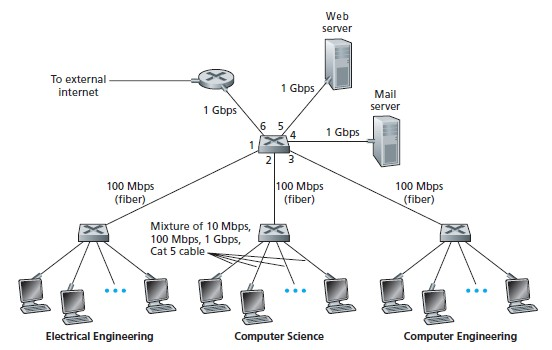
\includegraphics[width=0.95\linewidth]{cap20/switched_lan.png}
\end{minipage}\hfill
\begin{minipage}{0.46\linewidth}
È comune che le LAN usino uno o più switch per collegare molti dispositivi locali (nell'esempio del Kurose, i dipartimenti di un
istituto collegati da switch, con un router verso Internet e i server Web e di posta).
\end{minipage}
\caption{Una rete di istituto con switch organizzati ad albero (da Kurose).}
\end{figure}

A differenza dei router, gli switch sono \textbf{veloci} e \textbf{plug-and-play}:

\begin{itemize}
    \item non c'è alcun algoritmo di routing;
    \item si considerano solo i primi \textbf{2 livelli} della pila.
\end{itemize}

D'altra parte le LAN commutate sono \textbf{limitate in dimensione} e devono essere \textbf{strutturate ad albero}:

\begin{itemize}
    \item gli indirizzi MAC sono difficili da raggruppare (non hanno prefissi legati alla posizione): le tabelle degli switch possono crescere rapidamente;
    \item non c'è routing: i \textbf{cicli} sono difficili da evitare (un frame inondato in un ciclo girerebbe per sempre).
\end{itemize}

\subsection{Due cavi tra due switch}

Due switch sono collegati da due cavi, per ridondanza. Un host invia un frame a un indirizzo che nessuno dei due ha imparato. Che
succede? Ciascuno switch lo inonda su entrambi i cavi, riceve le copie dell'altro e le inonda di nuovo: il frame \textbf{gira per
sempre}.

\begin{itemize}
    \item Uno switch non sa distinguere una copia da un frame nuovo: niente nel frame dice che è già stato visto.
    \item E niente lo uccide mai: il frame Ethernet \textbf{non ha un TTL}. IP ne ha uno proprio perché un ciclo finisca, come ha
          mostrato traceroute.
    \item Un broadcast fa lo stesso su tutti i cicli contemporaneamente: è una \textbf{tempesta di broadcast} (\emph{broadcast
          storm}), e la LAN cade in pochi secondi.
\end{itemize}

\dfn{Spanning tree}{
    Si tengono i cavi ridondanti, ma se ne usa un \textbf{albero}: un solo percorso tra due stazioni qualsiasi, così nessun frame può
    tornare indietro.
    \begin{itemize}
      \item Gli switch si scambiano messaggi ed eleggono una \textbf{radice}: quello con l'identificatore più basso, costruito a
            partire dal suo indirizzo MAC.
      \item Ogni switch tiene il proprio percorso più breve verso la radice e \textbf{disattiva le porte} che non vi stanno sopra.
      \item Non smette mai di girare: se un cavo dell'albero si rompe, uno di quelli disattivati viene riattivato e l'albero
            ricostruito.
    \end{itemize}
    È l'algoritmo di \textbf{Radia Perlman}, standardizzato come IEEE \textbf{802.1D}. Gli switch eseguono quindi un algoritmo, ma non
    per scegliere percorsi: solo per \textbf{evitare i cicli}.
}

\begin{figure}[H]
\centering
\begin{tikzpicture}[every node/.style={font=\scriptsize\sffamily}]
  \node (s1) at (0,0) {\icon[1cm]{switch}}; \node[above=-2pt of s1] {S1: radice (ID più basso)};
  \node (s2) at (-2.6,-1.9) {\icon[1cm]{switch}}; \node[below=-2pt of s2] {S2};
  \node (s3) at (2.6,-1.9) {\icon[1cm]{switch}}; \node[below=-2pt of s3] {S3};
  \draw[wired, line width=1.6pt] (s1) -- (s2); \draw[wired, line width=1.6pt] (s1) -- (s3);
  \draw[black!35, dashed, line width=1.4pt] (s2) -- node[midway, text=netred, font=\bfseries\large] {$\times$} node[midway, below=5pt, text=netred] {porta disattivata} (s3);
  \node[text width=5cm, anchor=west] at (4.3,-0.9) {Il cavo S2--S3 resta collegato ma non porta frame; se cade S1--S3, lo spanning tree lo riattiva.};
\end{tikzpicture}
\caption{Tre switch in triangolo: lo spanning tree spegne un collegamento e resta un albero.}
\end{figure}

% ══════════════════════════════════════════════════════════════
\section{Switch o router}
% ══════════════════════════════════════════════════════════════

Entrambi sono commutatori di pacchetto \textbf{store-and-forward}: differiscono per \textbf{quanto in alto} nella pila guardano. Lo switch
si ferma al livello 2 e inoltra in base agli indirizzi MAC; il router sale al livello 3 e inoltra in base agli indirizzi IP. È ancora
una volta \emph{match più azione}, su un altro indirizzo in un altro header.

\begin{table}[H]
\centering
\begin{tabular}{p{3.5cm}p{5.2cm}p{5.2cm}}
\toprule
 & \textbf{Switch} & \textbf{Router} \\
\midrule
Livello & collegamento (2) & rete (3) \\
Indirizzi & MAC & IP \\
Tabelle & self-learning & algoritmi di routing \\
Configurazione & plug-and-play & va configurato \\
Topologia & albero (niente cicli) & qualsiasi, anche con cicli \\
Traffico broadcast & lo inoltra & lo blocca (separa i domini) \\
\bottomrule
\end{tabular}
\caption{Switch e router a confronto.}
\end{table}

\begin{table}[H]
\centering
\begin{tabular}{lccc}
\toprule
 & \textbf{Hub} & \textbf{Router} & \textbf{Switch} \\
\midrule
Isolamento del traffico & no & sì & sì \\
Plug and play & sì & no & sì \\
Instradamento ottimo & no & sì & no \\
\bottomrule
\end{tabular}
\caption{Quando usare che cosa.}
\end{table}

\begin{itemize}
    \item \textbf{Switch}: veloci e plug-and-play; ma la topologia in uso deve essere un albero, e un solo host guasto può inondare tutti
          di broadcast.
    \item \textbf{Router}: qualsiasi topologia e il percorso migliore, e un broadcast si ferma lì; ma ogni interfaccia ha bisogno di un
          indirizzo IP.
    \item Qualche centinaio di host: bastano gli switch. Migliaia: switch dentro ciascuna parte, router tra le parti.
\end{itemize}

% ══════════════════════════════════════════════════════════════
\section{Le VLAN}
% ══════════════════════════════════════════════════════════════

L'albero dipartimentale che abbiamo appena visto ha tre punti deboli:

\begin{itemize}
    \item \textbf{nessun isolamento}: i broadcast (ARP, DHCP, destinazioni sconosciute) attraversano l'intero istituto, e chiunque
          faccia sniffing li vede;
    \item \textbf{switch sprecati}: dieci piccoli dipartimenti richiedono dieci switch, dove ne basterebbe uno da 96 porte;
    \item \textbf{persone che si spostano}: un utente che cambia dipartimento va ricablato su un altro switch.
\end{itemize}

\dfn{VLAN basata sulle porte}{
    Le porte di un unico switch vengono divise in \textbf{gruppi}: ogni gruppo è una LAN separata, e un \textbf{dominio di broadcast}
    distinto. Tra due VLAN il traffico passa da un \textbf{router}, come tra due LAN, spesso dentro la stessa scatola.
}

\subsection{I trunk e il tag 802.1Q}

Due switch con VLAN in due edifici: un solo collegamento, il \textbf{trunk}, porta tutte le VLAN, invece di un cavo per VLAN. Ogni frame
sul trunk dichiara la propria VLAN con un \textbf{tag} di 4 byte, aggiunto e tolto dagli switch.

\begin{figure}[H]
\centering
\begin{tikzpicture}[every node/.style={font=\scriptsize\sffamily}]
  \node[anchor=east, font=\footnotesize\bfseries\sffamily, align=right] at (-0.2,0) {su una porta\\di accesso};
  \node[field, fill=lphy, minimum width=1.5cm] (p1) at (0.75,0) {preambolo};
  \node[field, fill=llink, minimum width=1.5cm, right=0pt of p1] (d1) {dest.};
  \node[field, fill=llink, minimum width=1.5cm, right=0pt of d1] (s1) {sorgente};
  \node[field, fill=lnet!50, minimum width=1.1cm, right=0pt of s1] (t1) {tipo};
  \node[field, fill=cloudbg, minimum width=3.2cm, right=0pt of t1] (x1) {dati};
  \node[field, fill=netred!25, minimum width=1cm, right=0pt of x1] {CRC};
  \begin{scope}[yshift=-1.2cm]
    \node[anchor=east, font=\footnotesize\bfseries\sffamily, align=right] at (-0.2,0) {su un\\trunk};
    \node[field, fill=lphy, minimum width=1.5cm] (p2) at (0.75,0) {preambolo};
    \node[field, fill=llink, minimum width=1.5cm, right=0pt of p2] (d2) {dest.};
    \node[field, fill=llink, minimum width=1.5cm, right=0pt of d2] (s2) {sorgente};
    \node[field, fill=netorange!40, minimum width=1.3cm, right=0pt of s2] (tp) {TPID 0x8100};
    \node[field, fill=netorange!40, minimum width=1.1cm, right=0pt of tp] (tc) {TCI};
    \node[field, fill=lnet!50, minimum width=1.1cm, right=0pt of tc] (t2) {tipo};
    \node[field, fill=cloudbg, minimum width=2.4cm, right=0pt of t2] (x2) {dati};
    \node[field, fill=netred!25, minimum width=1cm, right=0pt of x2] (c2) {CRC$'$};
    \node[right=2pt of c2, text=netred] {ricalcolato};
  \end{scope}
  \begin{scope}[yshift=-2.5cm]
    \node[field, fill=netorange!20, minimum width=1.6cm] (pr) at (4.9,0) {priorità};
    \node[field, fill=netorange!20, minimum width=0.4cm, right=0pt of pr] (cf) {1};
    \node[field, fill=netorange!20, minimum width=2.6cm, right=0pt of cf] (vi) {VLAN ID};
    \node[below=0pt of pr] {3 bit}; \node[below=0pt of vi] {12 bit};
    \draw[dashed, black!50] (tc.south west) -- (pr.north west); \draw[dashed, black!50] (tc.south east) -- (vi.north east);
    \node[anchor=west, text width=3.6cm] at (9.6,0) {il tag: 4 byte, aggiunti e tolti dagli switch};
  \end{scope}
\end{tikzpicture}
\caption{Il tag 802.1Q si inserisce tra l'indirizzo sorgente e il tipo.}
\end{figure}

\begin{itemize}
    \item Il VLAN ID ha 12 bit: al massimo \textbf{4094 VLAN} (due valori sono riservati). Il CRC copre anche il tag, quindi viene
          \textbf{ricalcolato} a entrambi gli estremi del trunk.
    \item \texttt{0x8100} sta esattamente dove stava il tipo: per un dispositivo che non sa nulla di VLAN, il frame porta un protocollo
          sconosciuto.
\end{itemize}

% ══════════════════════════════════════════════════════════════
\section{Il protocollo ARP}
% ══════════════════════════════════════════════════════════════

I protocolli dei livelli superiori lavorano con gli indirizzi IP, mentre il frame ha bisogno dell'indirizzo MAC del destinatario. Serve quindi
tradurre gli indirizzi IP in indirizzi MAC.

\dfn{ARP (Address Resolution Protocol)}{
    L'\textbf{ARP} gestisce la conversione tra indirizzi IP e indirizzi MAC.
    \begin{itemize}
      \item Ogni interfaccia ha un modulo ARP con una \textbf{tabella ARP}, che associa ogni IP della LAN a un indirizzo MAC, con un
            \textbf{TTL} (\emph{time to live}) scaduto il quale la voce viene cancellata (tipicamente 5--20 minuti).
      \item Poiché gli indirizzi MAC sono locali, anche ARP funziona \textbf{solo nelle reti locali}, cioè nella stessa subnet.
    \end{itemize}
    Il livello di rete consegna un datagramma e un indirizzo IP; il frame ha bisogno di un indirizzo MAC: ARP traduce.
}

\begin{table}[H]
\centering
\begin{tabular}{lll}
\toprule
\textbf{Indirizzo IP} & \textbf{Indirizzo MAC} & \textbf{TTL} \\
\midrule
222.222.222.221 & 88-B2-2F-54-1A-0F & 13:45:00 \\
222.222.222.223 & 5C-66-AB-90-75-B1 & 13:52:00 \\
\bottomrule
\end{tabular}
\caption{Una tabella ARP: la voce scade all'orario indicato.}
\end{table}

\info{ARP e DNS}{
    ARP fa per la LAN quello che il DNS fa per Internet: il DNS traduce \textbf{nomi} in indirizzi IP (in tutta Internet), ARP traduce
    \textbf{indirizzi IP} in indirizzi MAC (solo nella propria LAN). Come il DNS risolve un nome in un altro; a differenza del DNS,
    funziona solo sulla stessa subnet.
}

\subsection{La tabella ARP sulla propria macchina}

\begin{lstlisting}[language=bash]
$ ip neigh
192.168.1.1 dev enp3s0 lladdr 10:bd:18:e5:74:80 REACHABLE
192.168.1.17 dev enp3s0 lladdr 3c:52:82:4a:2b:91 STALE
$ sudo ip neigh flush dev enp3s0          # dimentica tutto
$ ping -c1 192.168.1.17 > /dev/null       # un datagramma, quindi prima un ARP
$ ip neigh show 192.168.1.17
192.168.1.17 dev enp3s0 lladdr 3c:52:82:4a:2b:91 REACHABLE
\end{lstlisting}

\begin{itemize}
    \item Al posto della colonna di scadenza c'è uno \textbf{stato}: \texttt{REACHABLE} è stato appena confermato, \texttt{STALE} è
          ancora usato e verrà ricontrollato al prossimo bisogno. In ogni caso una voce scade: un host che se ne va sparisce da ogni
          tabella da solo.
    \item Dopo il \texttt{flush} il ping ha dovuto aspettare uno scambio ARP; ne guarderemo uno alla fine del capitolo.
    \item È anche il modo in cui \texttt{nmap -sn} trova gli host della propria subnet: una richiesta per indirizzo, e per questo
          riporta anche gli indirizzi MAC.
\end{itemize}

\subsection{Un esempio di ARP}

\begin{figure}[H]
\centering
\begin{minipage}{0.44\linewidth}\centering
  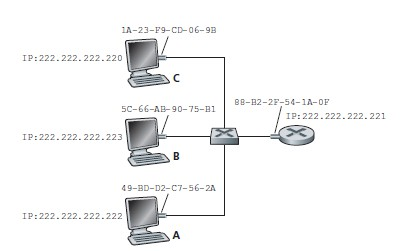
\includegraphics[width=0.95\linewidth]{cap20/arp_lan.png}
\end{minipage}\hfill
\begin{minipage}{0.52\linewidth}
L'host C (\texttt{222.222.222.220}) vuole inviare messaggi all'host A (\texttt{222.222.222.222}). Per farlo deve conoscere anche il MAC di A.
\begin{enumerate}
  \item Se A \textbf{non è nella tabella}, prima di inviare il messaggio C invia in \textbf{broadcast} a tutti i dispositivi della rete un
        pacchetto \textbf{ARP request}: ``chi ha l'IP \texttt{222.222.222.222}? Lo dica a \texttt{222.222.222.220}''.
  \item Tutti i nodi ricevono il pacchetto, ma \textbf{solo} chi ha l'IP cercato risponde, con un messaggio \textbf{ARP reply} diretto
        (\emph{unicast}) che contiene il proprio MAC.
  \item C inserisce la coppia IP--MAC nella propria tabella e invia il frame.
\end{enumerate}
\end{minipage}
\caption{ARP in una LAN: tre host e un router collegati da uno switch (da Kurose).}
\end{figure}

\begin{figure}[H]
\centering
\begin{tikzpicture}[yscale=0.85, every node/.style={font=\scriptsize\sffamily}]
  \timeline{c}{0}{C}{3.6}
  \timeline{b}{4}{B}{3.6}
  \timeline{a}{8}{A}{3.6}
  \draw[msg, netred] (0,-0.5) -- node[above, sloped, pos=0.5] {ARP request (dest. FF-FF-FF-FF-FF-FF): chi ha 222.222.222.222?} (8,-0.5);
  \fill[netred] (4,-0.5) circle (2.5pt); \node[anchor=west, text=netred] at (4.1,-0.85) {riceve e ignora};
  \node[anchor=west] at (8.2,-0.5) {``sono io!''};
  \draw[msg, netgreen!60!black] (8,-1.7) -- node[above, pos=0.5] {ARP reply (unicast): 222.222.222.222 è 49-BD-D2-C7-56-2A} (0,-1.7);
  \node[anchor=east, text width=2.6cm, align=right] at (-0.2,-1.9) {aggiorna la tabella ARP};
  \draw[msg, netblue, very thick] (0,-2.8) -- node[above] {frame IP con MAC di destinazione di A} (8,-2.8);
\end{tikzpicture}
\caption{Richiesta in broadcast, risposta in unicast.}
\end{figure}

Perché la richiesta va in broadcast e la risposta no? Chi chiede non conosce il MAC del destinatario (è proprio ciò che cerca), quindi
non può che chiedere a tutti; chi risponde conosce il MAC di chi ha chiesto, perché la richiesta lo contiene.

\subsection{Un pacchetto ARP}

\begin{table}[H]
\centering
\begin{tabular}{lclll}
\toprule
\textbf{Campo} & \textbf{Byte} & \textbf{Richiesta da C} & \textbf{Risposta da A} \\
\midrule
hardware, protocollo, lunghezze & 6 & Ethernet, IPv4, 6, 4 & gli stessi \\
operazione & 2 & 1, richiesta & 2, risposta \\
MAC del mittente & 6 & quello di C & quello di A \\
IP del mittente & 4 & 222.222.222.220 & 222.222.222.222 \\
MAC del destinatario & 6 & sconosciuto: zeri & quello di C \\
IP del destinatario & 4 & 222.222.222.222 & 222.222.222.220 \\
\bottomrule
\end{tabular}
\caption{I campi di un pacchetto ARP: 28 byte in tutto.}
\end{table}

\begin{itemize}
    \item Viaggia direttamente in un frame Ethernet di tipo \texttt{0x0806}: niente header IP, niente porte.
    \item Contiene indirizzi di entrambi i livelli, quindi appartiene a tutti e due e a nessuno: ARP sta \textbf{a cavallo} del confine
          tra rete e collegamento.
    \item L'intero pacchetto è di \textbf{28 byte}: teniamo a mente il numero per la lunghezza minima del frame.
\end{itemize}

\warning{Nessuno controlla la risposta}{
    Una risposta ARP dice che \texttt{192.168.1.1} ha un certo indirizzo MAC. Chi verifica che sia vero? \textbf{Nessuno}: ARP non ha
    autenticazione, e gli host accettano anche risposte che non hanno mai chiesto. Le risposte non richieste hanno un uso onesto: un
    host che entra nella rete annuncia la propria associazione, un \textbf{gratuitous ARP}. Ma un attaccante può annunciare l'IP del
    \textbf{gateway} con il proprio MAC (\textbf{ARP poisoning}, o \emph{ARP spoofing}): ogni host aggiorna la tabella e gli manda il
    traffico diretto all'esterno. L'attaccante inoltra tutto, così nulla sembra rotto: un \emph{man in the middle}, uno degli attacchi
    più comuni in una LAN. Le difese stanno fuori da ARP: una voce statica per il gateway, switch che controllano ogni risposta
    rispetto a ciò che il DHCP ha assegnato (\emph{Dynamic ARP Inspection}).
}

\subsection{ARP e il gateway}

Che succede se l'IP di destinazione è \textbf{fuori dalla rete}?

\begin{figure}[H]
    \centering
    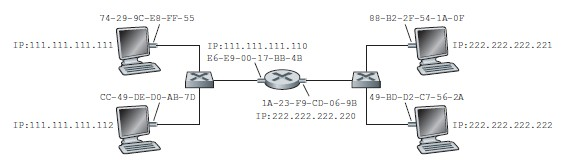
\includegraphics[width=0.7\linewidth]{cap20/arp_gateway.png}
    \caption{Due subnet (111.111.111.x e 222.222.222.x) collegate da un router con due interfacce, ciascuna con il proprio IP, MAC e tabella ARP.}
\end{figure}

\begin{itemize}
    \item Il router che collega le due reti deve avere almeno \textbf{2 interfacce} (2 IP, 2 MAC e 2 tabelle ARP), una dentro ciascuna subnet.
    \item I frame diretti fuori dalla subnet vengono inviati alla \textbf{prima interfaccia del router}: l'host usa ARP per il MAC del
          \textbf{router} (il gateway), non per quello del destinatario finale.
    \item Il router estrae il datagramma, lo sposta sulla seconda interfaccia e, con la seconda tabella ARP, lo invia all'host giusto in un
          \textbf{nuovo frame}.
\end{itemize}

\begin{esempio}{Da A (111.111.111.111) a B (222.222.222.222)}
\begin{enumerate}
    \item A capisce, confrontando indirizzo e maschera, che B è in un'altra subnet: deve passare dal gateway \texttt{111.111.111.110}.
    \item A usa ARP per trovare il MAC dell'interfaccia del router \texttt{111.111.111.110} (\texttt{E6-E9-00-17-BB-4B}).
    \item A crea un datagramma IP con \textbf{IP sorgente A} e \textbf{IP destinazione B}, e lo incapsula in un frame con
          \textbf{MAC destinazione = MAC del router}.
    \item Il router riceve il frame, estrae il datagramma, vede che B è sulla subnet \texttt{222.222.222.0/24}, usa ARP su quell'interfaccia per
          trovare il MAC di B e crea un nuovo frame con \textbf{MAC sorgente = sua seconda interfaccia} e \textbf{MAC destinazione = B}.
\end{enumerate}
Se A scrivesse nel frame il MAC di B, \texttt{49-BD-D2-C7-56-2A}, nessun adattatore della subnet di sinistra corrisponderebbe e il
frame verrebbe scartato da tutti.
\begin{center}
\begin{tabular}{lll}
\toprule
 & \textbf{Frame nella subnet di sinistra} & \textbf{Frame nella subnet di destra} \\
\midrule
MAC sorgente & \texttt{74-29-9C-E8-FF-55} (A) & \texttt{1A-23-F9-CD-06-9B} (router, if. 2) \\
MAC destinazione & \texttt{E6-E9-00-17-BB-4B} (router, if. 1) & \texttt{49-BD-D2-C7-56-2A} (B) \\
IP sorgente & \texttt{111.111.111.111} & \texttt{111.111.111.111} \\
IP destinazione & \texttt{222.222.222.222} & \texttt{222.222.222.222} \\
\bottomrule
\end{tabular}
\end{center}
\end{esempio}

\begin{itemize}
    \item Gli indirizzi \textbf{IP} sono scritti una volta, dal mittente, e arrivano invariati: nominano i due estremi del
          \textbf{percorso}.
    \item Gli indirizzi \textbf{MAC} sono riscritti da ogni router: nominano i due estremi di \textbf{un collegamento}.
    \item Ogni hop costa quindi una ricerca in una tabella ARP. La traduzione degli indirizzi dal lato IP (il NAT) è l'eccezione, ed è
          voluta.
\end{itemize}

% ══════════════════════════════════════════════════════════════
\section{Il frame Ethernet}
% ══════════════════════════════════════════════════════════════

Ethernet è la tecnologia dominante per le LAN cablate. La sua storia è quella di un cavo coassiale diventato uno switch:

\begin{itemize}
    \item Bob \textbf{Metcalfe} e David \textbf{Boggs} costruirono Ethernet allo Xerox PARC a metà degli anni '70, dopo che Metcalfe aveva
          passato tre mesi con ALOHAnet.
    \item \textbf{Il bus}: un cavo coassiale lungo l'edificio, con le stazioni agganciate sopra: una LAN broadcast, governata dal CSMA/CD
          che abbiamo ricavato.
    \item \textbf{L'hub}: alla fine degli anni '90, doppini intrecciati a stella attorno a un hub: più facile da cablare e da riparare,
          logicamente lo stesso cavo.
    \item \textbf{Lo switch}: nei primi anni 2000 l'hub è diventato uno switch: ancora una stella, ora store-and-forward e senza
          collisioni, con collegamenti full-duplex.
    \item Token ring, FDDI, ATM hanno fatto meglio per un po'. Ethernet ha vinto arrivando per primo, costando poco e recuperando
          sempre in velocità.
\end{itemize}

\begin{figure}[H]
\centering
\begin{tikzpicture}[every node/.style={font=\scriptsize\sffamily}]
  \node[anchor=east, font=\footnotesize\bfseries\sffamily] at (-0.2,0) {Ethernet (DIX)};
  \node[field, fill=lphy, minimum width=1.6cm] (pr) at (0.8,0) {preambolo};
  \node[field, fill=llink, minimum width=1.9cm, right=0pt of pr] (dst) {indirizzo dest.};
  \node[field, fill=llink, minimum width=1.9cm, right=0pt of dst] (src) {indirizzo sorg.};
  \node[field, fill=lnet!50, minimum width=0.9cm, right=0pt of src] (ty) {tipo};
  \node[field, fill=cloudbg, minimum width=3.2cm, right=0pt of ty] (da) {dati};
  \node[field, fill=cloudbg!50, minimum width=0.9cm, right=0pt of da] (pad) {pad};
  \node[field, fill=netred!25, minimum width=1.3cm, right=0pt of pad] (crc) {CRC};
  \foreach \n/\b in {pr/8, dst/6, src/6, ty/2, da/{0--1500}, pad/{0--46}, crc/4} \node[above=0pt of \n] {\b};
  \node[anchor=east] at (-0.2,0.45) {byte};
  \begin{scope}[yshift=-1.1cm]
    \node[anchor=east, font=\footnotesize\bfseries\sffamily] at (-0.2,0) {IEEE 802.3};
    \node[field, fill=lphy, minimum width=1.3cm] (pr2) at (0.65,0) {preambolo};
    \node[field, fill=lphy!60, minimum width=0.3cm, right=0pt of pr2] (sof) {\rotatebox{90}{\tiny SOF}};
    \node[field, fill=llink, minimum width=1.9cm, right=0pt of sof] (dst2) {indirizzo dest.};
    \node[field, fill=llink, minimum width=1.9cm, right=0pt of dst2] (src2) {indirizzo sorg.};
    \node[field, fill=lnet!50, minimum width=0.9cm, right=0pt of src2] (ln) {lungh.};
    \node[field, fill=cloudbg, minimum width=3.2cm, right=0pt of ln] {dati};
    \node[field, fill=cloudbg!50, minimum width=0.9cm] at (9.95,0) {pad};
    \node[field, fill=netred!25, minimum width=1.3cm] at (11.05,0) {CRC};
  \end{scope}
\end{tikzpicture}
\caption{Il frame Ethernet nelle due varianti (DIX e IEEE 802.3).}
\end{figure}

\begin{itemize}
    \item \textbf{Preambolo} (8 byte): sette byte \texttt{10101010} agganciano l'orologio del ricevente; poi \texttt{10101011}, in cui i
          due 1 finali dicono ``via'' (lo \emph{start frame delimiter}).
    \item \textbf{Indirizzo di destinazione} (6 byte): il MAC dell'adattatore di destinazione. Sta \textbf{per primo}, così uno switch può
          cominciare a inoltrare prima che il frame sia arrivato del tutto.
    \item \textbf{Indirizzo sorgente} (6 byte): il MAC dell'adattatore che ha messo il frame su questo collegamento.
    \item \textbf{Tipo} (2 byte): a chi consegnare i dati: \texttt{0x0800} IPv4, \texttt{0x0806} ARP, \texttt{0x86DD} IPv6. Come il campo
          protocollo di IP.
    \item \textbf{Dati} (da 46 a 1500 byte): il datagramma. 1500 è la \textbf{MTU} di Ethernet: se il datagramma è più grande, va
          frammentato. L'intero frame arriva a 1518 byte.
    \item \textbf{Pad}: riempimento per raggiungere la lunghezza minima dei dati (46 byte).
    \item \textbf{CRC} (4 byte): il CRC-32 costruito sui polinomi, calcolato dall'indirizzo di destinazione ai dati; il preambolo non è
          coperto.
\end{itemize}

\subsection{Tipo o lunghezza}

DIX (Digital, Intel, Xerox) ha messo un \textbf{tipo} in quei due byte; IEEE 802.3 ha messo una \textbf{lunghezza} nello stesso posto.
Le due forme si distinguono \textbf{dal valore}: ogni tipo mai assegnato è sopra 1500 (da \texttt{0x0600} in su), e una lunghezza
non supera 1500. Quasi tutto il traffico è DIX, che Wireshark chiama \textbf{Ethernet II}. La forma con la lunghezza sopravvive in
pochi frame (tra cui i messaggi dello spanning tree), con un header in più all'interno per dire che cosa portano.

\subsection{Perché i frame corti vengono riempiti}

Un pacchetto ARP è di 28 byte; indirizzi, tipo e CRC ne aggiungono 18. Che cosa va sul filo? Un frame di 46 byte sarebbe troppo corto
per essere sicuri di sentire una collisione: l'adattatore aggiunge \textbf{18 byte di pad}, e il frame è di \textbf{64}.

\begin{itemize}
    \item I 64 byte dalla destinazione al CRC sono i \textbf{512 bit} richiesti dall'argomento del $2\tau$, scritti nel formato.
    \item Da qui il campo dati minimo di 46 byte: $64 - 6 - 6 - 2 - 4$.
    \item Il ricevente consegna dati e pad insieme. Il protocollo superiore conosce la propria lunghezza (IP dal campo
          \emph{total length}) e scarta il resto.
    \item Il formato ha mantenuto quel minimo anche sui collegamenti commutati, dove non collide più niente.
\end{itemize}

\info{Un servizio senza connessione e inaffidabile}{
    Ethernet è \textbf{senza connessione} (nessun handshake con l'adattatore di destinazione) e \textbf{inaffidabile}: il ricevente non invia né ACK
    né NAK. Un frame che non supera il controllo CRC viene semplicemente scartato; se i dati servono davvero, sarà TCP (o l'applicazione)
    ad accorgersi della mancanza e a ritrasmettere, attraverso lo stesso adattatore, che non sa distinguere una ritrasmissione da
    qualsiasi altra cosa.
}

\subsection{Quarant'anni, un solo formato di frame}

I nomi delle varianti si leggono così: \textbf{10BASE-T}, \textbf{100BASE-TX}, \textbf{1000BASE-LX}, \textbf{10GBASE-T}: la velocità,
\textbf{BASE} per i mezzi dedicati solo a Ethernet (banda base), poi il mezzo (T doppino, LX fibra a onda lunga, \dots). Da 10 Mb/s a
centinaia di Gb/s, su coassiale, rame e fibra, il livello fisico è cambiato più e più volte, e il frame no. Velocità, mezzi,
topologia, perfino il protocollo di accesso sono stati sostituiti: ciò che è ancora Ethernet è il \textbf{formato del frame}.

% ══════════════════════════════════════════════════════════════
\section{La nostra chat, un livello più in basso}
% ══════════════════════════════════════════════════════════════

Il server della chat gira su \texttt{.17}, il client qui su \texttt{.23}. Con l'opzione \texttt{-e} tcpdump stampa anche l'header
Ethernet:

\begin{lstlisting}[language=bash]
$ sudo tcpdump -i enp3s0 -t -e -n 'port 5000'
3c:52:82:4a:1f:07 > 3c:52:82:4a:2b:91, ethertype IPv4 (0x0800), length 74: ... Flags [S]
3c:52:82:4a:2b:91 > 3c:52:82:4a:1f:07, ethertype IPv4 (0x0800), length 74: ... Flags [S.]
3c:52:82:4a:1f:07 > 3c:52:82:4a:2b:91, ethertype IPv4 (0x0800), length 66: ... Flags [.]
3c:52:82:4a:1f:07 > 3c:52:82:4a:2b:91, ethertype IPv4 (0x0800), length 76: ... Flags [P.]
\end{lstlisting}

\begin{itemize}
    \item Prima della virgola c'è il livello di collegamento: due adattatori e il tipo \texttt{0x0800}. Niente di tutto ciò è nel
          nostro codice.
    \item \texttt{length 76}: 14 byte di Ethernet, 20 di IP, 32 di TCP (con le opzioni), e dal byte 66 il nostro header,
          \texttt{00 00 00 05 02} (quattro byte di lunghezza e uno di tipo), poi \texttt{hello}.
    \item Su loopback Linux stampa un header Ethernet di zeri: non è uscito nulla dalla macchina, e il kernel finge.
    \item Su Wi-Fi si vede comunque Ethernet II: il driver ha già tradotto i frame radio prima che la cattura li veda.
\end{itemize}

\subsection{Prima del primo SYN}

Si svuota la tabella ARP, poi si avvia il client. Qual è il primo frame sul filo? Non il SYN: il kernel non può costruire un frame per
il server prima di conoscerne il MAC, quindi va prima uno scambio ARP.

\begin{lstlisting}[language=bash]
$ sudo tcpdump -i enp3s0 -t -e -n 'arp or port 5000'
3c:52:82:4a:1f:07 > ff:ff:ff:ff:ff:ff, ethertype ARP (0x0806), length 42: Request who-has 192.168.1.17
3c:52:82:4a:2b:91 > 3c:52:82:4a:1f:07, ethertype ARP (0x0806), length 60: Reply 192.168.1.17 is-at ...
3c:52:82:4a:1f:07 > 3c:52:82:4a:2b:91, ethertype IPv4 (0x0800), length 74: ... Flags [S]
\end{lstlisting}

\begin{itemize}
    \item La richiesta va a tutti uni, la risposta torna al solo nostro adattatore. Poi, e solo poi, l'handshake.
    \item Server su un'altra subnet? L'ARP è per il gateway, e il MAC del server non attraversa mai il nostro filo.
\end{itemize}

\warning{Un frame più corto del minimo}{
    La richiesta è uscita a 42 byte, e il minimo è 64. Il nostro adattatore viola la regola? No: la cattura vede il frame
    \textbf{prima} che l'adattatore lo completi. I 18 byte di pad e i 4 di CRC vengono aggiunti sotto il punto in cui guarda il software.
    La risposta è arrivata a 60: riempita dall'altro adattatore, con il CRC controllato e tolto dal nostro. Il preambolo non si vede
    mai: una cattura comincia dall'indirizzo di destinazione. E tra due macchine virtuali entrambe possono leggere 42: nessun
    adattatore reale le ha toccate. Il campo che esiste per la velocità della luce è proprio quello che gli strumenti non possono
    mostrare: la regola del $2\tau$ vive nell'hardware.
}

\begin{esercizio}{Indirizzi, switch e frame}
\begin{enumerate}[label=(\alph*)]
    \item Per ciascuno dei primi byte \texttt{00}, \texttt{01}, \texttt{02}, \texttt{3c}, \texttt{f2}, \texttt{ff} dire se l'indirizzo è
          unicast o di gruppo, universale o locale.
    \item Calcolare l'indirizzo MAC multicast dei gruppi \texttt{239.1.2.3} e \texttt{224.129.2.3}. Che cosa si nota?
    \item Uno switch a 4 porte ha la tabella vuota; A è sulla porta 1, B sulla 2, C sulla 3, e sulla porta 4 c'è un hub con D ed E.
          Passano nell'ordine i frame A$\rightarrow$B, D$\rightarrow$A, E$\rightarrow$D, B$\rightarrow$E. Per ciascuno dire che cosa
          fa lo switch e che cosa impara.
    \item Quanto è lungo sul filo, preambolo escluso, un frame Ethernet che porta un datagramma IP di 30 byte? E uno di 1500?
\end{enumerate}

\svolgimento
\begin{enumerate}[label=(\alph*)]
    \item Si guardano i due bit meno significativi del primo byte (gruppo, poi locale). \texttt{00}: unicast, universale.
          \texttt{01}: gruppo, universale (è il prefisso multicast \texttt{01-00-5E}). \texttt{02}: unicast, locale. \texttt{3c}
          $=$ \texttt{00111100}: unicast, universale. \texttt{f2} $=$ \texttt{11110010}: unicast, locale. \texttt{ff}: gruppo e
          locale, ed è il broadcast.
    \item Si prendono i 23 bit bassi: per \texttt{239.1.2.3} il secondo byte è 1 $=$ \texttt{0000\,0001}, si tiene \texttt{000\,0001},
          quindi \texttt{01-00-5E-01-02-03}. Per \texttt{224.129.2.3} il secondo byte è 129 $=$ \texttt{1000\,0001}: il bit alto si
          perde, resta ancora \texttt{000\,0001}, e l'indirizzo è \textbf{lo stesso}, \texttt{01-00-5E-01-02-03}. Sono due dei 32
          gruppi che condividono quell'indirizzo.
    \item A$\rightarrow$B: impara A sulla 1; B sconosciuto, inonda su 2, 3, 4. D$\rightarrow$A: impara D sulla 4; A è sulla 1,
          inoltra solo lì. E$\rightarrow$D: impara E sulla 4; D è sulla 4, la stessa porta da cui è arrivato il frame: lo
          \textbf{filtra} (D l'ha già ricevuto dall'hub). B$\rightarrow$E: impara B sulla 2; E è sulla 4, inoltra solo lì.
    \item 30 byte di dati sono meno di 46: si aggiungono 16 byte di pad, e il frame è di $6 + 6 + 2 + 46 + 4 = 64$ byte. Con 1500
          byte di dati il frame è di $6 + 6 + 2 + 1500 + 4 = 1518$ byte, il massimo.
\end{enumerate}
\end{esercizio}

\Needspace{20\baselineskip}
% ══════════════════════════════════════════════════════════════
\section{Riepilogo}
% ══════════════════════════════════════════════════════════════

\riepilogo{
\begin{itemize}
    \item L'\textbf{indirizzo MAC} (48 bit, piatto, OUI del produttore nei primi 24) identifica un'interfaccia ed è \textbf{locale};
          broadcast = \texttt{FF-FF-FF-FF-FF-FF}, multicast \texttt{01-00-5E} più 23 bit del gruppo.
    \item Gli \textbf{switch} inoltrano frame in base al MAC con una tabella imparata dagli indirizzi sorgente, inondano il resto, ed
          eliminano le collisioni (un dominio per porta); serve uno \textbf{spanning tree} per sopravvivere a un ciclo.
    \item Le \textbf{VLAN} dividono una rete commutata in più domini di broadcast; un tag 802.1Q di 4 byte porta la VLAN su un trunk.
    \item \textbf{ARP} traduce IP in MAC: richiesta in broadcast, risposta in unicast, tabella con TTL; vulnerabile all'\textbf{ARP poisoning}.
    \item Verso un'altra subnet il frame va al MAC del \textbf{router}: gli IP restano uguali, i MAC cambiano a ogni hop.
    \item \textbf{Frame Ethernet}: preambolo (8), destinazione (6), sorgente (6), tipo (2), dati (46--1500, con pad), CRC (4): da 64 a
          1518 byte. Il frame è sopravvissuto a ogni Ethernet.
\end{itemize}
}
